\part{Other Topics}
\chapter{Proofs}
\section{Induction}
\begin{theorem}[Principle of Mathematical Induction (PMI)]
Let $P(n)$ be a family of statements indexed by $\ZZ^+$. Suppose that 
\begin{enumerate}[label=(\roman*)]
\item (\textbf{base case}) $P(1)$ is true and
\item (\textbf{inductive step}) for all $k\in\ZZ^+$, $P(k)\implies P(k+1)$.
\end{enumerate}
Then $P(n)$ is true for all $n\in\ZZ^+$.
\end{theorem}

\begin{exercise}
Prove that for all positive integers $n$,
\[ 1+2+3+\cdots+n=\frac{n(n+1)}{2}. \]
\end{exercise}
\begin{proof}
The statement is true for $n=1$ (base case) because with $n=1$, LHS = RHS = $1$.

Assume that the statement is true for some $n=k$, where $k \in \ZZ^{+}$. By our induction hypothesis, we have $1 + 2 + 3 + \cdots + k = \dfrac{k(k+1)}{2}$.

To show that the statement is true for $k+1$, 
\begin{align*}
1 + 2 + 3 + \cdots + k + (k+1) &= \frac{k(k+1)}{2} + (k+1)\\
&= \frac{(k+1)(k+2)}{2}\\
&= \frac{(k+1)[(k+1)+1]}{2}
\end{align*}

Since $P(1)$ is true and $P(k)\implies P(k+1)$, by mathematical induction, $P(n)$ is true for all positive integers $n$.
\end{proof}

Another variant on induction is when the inductive step relies on some earlier case(s) but not necessarily the immediately previous case. This is known as \emph{strong induction}:

\begin{theorem}[Strong Form of Induction]
Let $P(n)$ be a family of statements indexed by the natural numbers. Suppose that
\begin{enumerate}[label=(\roman*)]
\item (\textbf{base case}) $P(1)$ is true and
\item (\textbf{inductive step}) for all $m \in \ZZ^+$, if for integers $k$ with $1 \le k \le m$, $P(k)$ is true then $P(m+1)$ is true.
\end{enumerate}
Then $P(n)$ is true for all $n \in \NN$.
\end{theorem}

\begin{theorem}[Cauchy Induction]
Let $P(n)$ be a family of statements indexed by $\ZZ^+_{\ge2}$. Suppose that
\begin{enumerate}[label=(\roman*)]
\item (\textbf{base case}) $P(2)$ is true and
\item (\textbf{inductive step}) for all $k\in\ZZ^+$, $P(k)\implies P(2k)$ and $P(k)\implies (k-1)$.
\end{enumerate}
Then $P(n)$ is true for all $n\in\ZZ^+_{\ge2}$.
\end{theorem}

\chapter{Riemann Integrals}
\section{Riemann Sums}
\vocab{Riemann sums} are an infinite sequence of sums that converges to an integral.

Given $y=f(x)$, we want to find the integral on the $x$-interval $[0,1]$.

We first split the interval $[0,1]$ into $n$ equal subintervals \[ \left[0, \frac{1}{n}\right], \left[\frac{1}{n}, \frac{2}{n}\right], \cdots, \left[\frac{n-1}{n}, 1\right] \]
as shown in the figure below.

\begin{figure}[H]
    \centering
    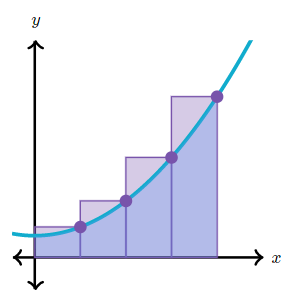
\includegraphics[width=0.25\linewidth]{images/Riemanns_sums.png}
    \label{fig:riemann-sum}
    \caption{Riemann sum}
\end{figure}

Considering the height of the rectangles, there is not much difference between choosing the left and right values, but the right value is usually chosen because it's simpler for calculation. Hence for the $k$-th subinterval $\sqbrac{\dfrac{k-1}{n}, \dfrac{k}{n}}$ where $k=1,\dots,n$, the height of rectangle is $f\brac{\dfrac{k}{n}}$. Thus the area of the $k$-th rectangle is given by
\[ \frac{1}{n} f\left(\frac{k}{n}\right).\]

Therefore, the integral is obtained by summing up the area of $n$ rectangles; that is,
\begin{equation} 
\int_{0}^{1} f(x) \dd{x} = \lim_{n \to \infty} \sum_{k=1}^{n} \frac{1}{n} f\brac{\frac{k}{n}}.
\end{equation}

\begin{exercise}
Find the values of the following expressions:
\begin{enumerate}[label=(\alph*)]
\item $\displaystyle\lim_{n\to\infty}\brac{\frac{1}{n+1}+\frac{1}{n+2}+\cdots+\frac{1}{2n}}$
\item $\displaystyle\lim_{n\to\infty}\frac{1}{n}\brac{e^\frac{1}{n}+e^\frac{2}{n}+\cdots+e^1}$
\item $\displaystyle\lim_{n\to\infty}\frac{\sqrt{n+1}+\sqrt{n+2}+\cdots+\sqrt{2n}}{n\sqrt{n}}$
\item $\displaystyle\lim_{n\to\infty}\brac{\frac{1}{\sqrt{n(n+1)}}+\frac{1}{\sqrt{n(n+2}}+\cdots+\frac{1}{\sqrt{n(4n)}}}$
\item $\displaystyle\lim_{n\to\infty}\frac{1}{n}\brac{\frac{1}{\sqrt{n^2}}+\frac{1}{\sqrt{n^2+1}}+\cdots+\frac{1}{\sqrt{2n^2}}}$
\end{enumerate}
\end{exercise}

\begin{solution} \ 
\begin{enumerate}[label=(\alph*)]
\item \begin{align*}
&\lim_{n\to\infty}\brac{\frac{1}{n+1}+\frac{1}{n+2}+\cdots+\frac{1}{2n}} \\
&= \lim_{n\to\infty}\frac{1}{n}\brac{\frac{1}{1+\frac{1}{n}}+\frac{1}{1+\frac{2}{n}}+\cdots+\frac{1}{1+\frac{n}{n}}} \\
&= \int_0^1\frac{1}{1+x}\dd{x}=\sqbrac{\ln(1+x)}_0^1=\boxed{\ln2}
\end{align*}
Note that in this case $f(x)=\dfrac{1}{1+x}$.

\item \begin{align*}
&\lim_{n\to\infty}\frac{1}{n}\brac{e^\frac{1}{n}+e^\frac{2}{n}+\cdots+e^1} \\
&= \int_0^1e^x\dd{x}=\sqbrac{e^x}_0^1=\boxed{e-1}
\end{align*}
Note that in this case $f(x)=e^x$.

\item \begin{align*}
&\lim_{n\to\infty}\frac{\sqrt{n+1}+\sqrt{n+2}+\cdots+\sqrt{2n}}{n\sqrt{n}} \\
&= \lim_{n\to\infty}\frac{1}{n}\brac{\sqrt{1+\frac{1}{n}}+\sqrt{1+\frac{2}{n}}+\cdots+\sqrt{1+\frac{n}{n}}} \\
&= \int_0^1\sqrt{1+x}\dd{x}=\sqbrac{\frac{2}{3}(1+x)^\frac{3}{2}}_0^1=\boxed{\frac{2}{3}(2\sqrt{2}-1)}
\end{align*}
Note that in this case $f(x)=\sqrt{1+x}$.

\item \begin{align*}
&\lim_{n\to\infty}\brac{\frac{1}{\sqrt{n(n+1)}}+\frac{1}{\sqrt{n(n+2}}+\cdots+\frac{1}{\sqrt{n(4n)}}} \\
&= \lim_{n\to\infty}\sum_{k=1}^{3n}\frac{1}{n}\brac{\frac{1}{\sqrt{1+\frac{k}{n}}}} \\
&= \int_0^3\frac{1}{\sqrt{1+x}}\dd{x}=\sqbrac{2\sqrt{1+x}}_0^3=\boxed{2}
\end{align*}
Note that the sum itself is the sum of $3n$ rectangles, with their heights determined by $f(x)$ from $x=0$ to $x=3$.

\item \begin{align*}
&\lim_{n\to\infty}\frac{1}{n}\brac{\frac{1}{\sqrt{n^2}}+\frac{1}{\sqrt{n^2+1}}+\cdots+\frac{1}{\sqrt{2n^2}}} \\
&= \lim_{n\to\infty}\frac{1}{n^2}\brac{\frac{1}{\sqrt{1+\frac{1}{n^2}}}+\frac{1}{\sqrt{1+\frac{2}{n^2}}}+\cdots+\frac{1}{\sqrt{1+\frac{n^2}{n^2}}}} \\
&= \int_0^1\frac{1}{\sqrt{1+x}}\dd{x}=\sqbrac{2\sqrt{1+x}}_0^1=\boxed{2\brac{\sqrt{2}-1}}
\end{align*}
Note that the interval $[0,1]$ is divided into $n^2$ subintervals.
\end{enumerate}
\end{solution}

\begin{exercise} \
\begin{enumerate}[label=(\alph*)]
\item Prove that for any positive integer $n\ge2$,
\[ 2\sqrt{n}-2<1+\frac{1}{\sqrt{2}}+\frac{1}{\sqrt{3}}+\cdots+\frac{1}{\sqrt{n}}<2\sqrt{n}-1. \]
\item Compare the sizes between $\displaystyle1+\frac{1}{\sqrt{2}}+\frac{1}{\sqrt{3}}+\cdots+\frac{1}{\sqrt{n}}$ and $2\sqrt{n}-\dfrac{3}{2}$.
\item Find the integer part of $\displaystyle1+\frac{1}{\sqrt{2}}+\frac{1}{\sqrt{3}}+\cdots+\frac{1}{\sqrt{2023}}$.
\end{enumerate}
\end{exercise}

\begin{solution} \
\begin{enumerate}[label=(\alph*)]
\item The sum $\displaystyle1+\frac{1}{\sqrt{2}}+\frac{1}{\sqrt{3}}+\cdots+\frac{1}{\sqrt{n}}$ is relevant area under the graph $y=\dfrac{1}{x}$, in the interval $[1,n]$. By integration, this area is $2\sqrt{n}-2$.

On the other hand, consider the area to be approximated by rectangles under the graph, then this approximation is $\displaystyle\frac{1}{\sqrt{2}}+\frac{1}{\sqrt{3}}+\cdots+\frac{1}{\sqrt{n}}$. Because all these rectangles are under the graph, we have
\[ \frac{1}{\sqrt{2}}+\frac{1}{\sqrt{3}}+\cdots+\frac{1}{\sqrt{n}}<2\sqrt{n}-2 \]
or
\[ 1+\frac{1}{\sqrt{2}}+\frac{1}{\sqrt{3}}+\cdots+\frac{1}{\sqrt{n}}<2\sqrt{n}-1. \]

Consider these rectangles to cover the area under the graph. The same area can be covered if we consider the slightly higher rectangles which use the $f$-value of each of the left endpoints. So we have $\displaystyle1+\frac{1}{\sqrt{2}}+\frac{1}{\sqrt{3}}+\cdots+\frac{1}{\sqrt{n-1}}>2\sqrt{n}-2$.

\item Consider the sum of trapeziums instead of just rectangles.

For each interval $[k,k+1]$, we use $f(k)$ and $f(k+1)$ for the two heights of the trapezium. Thus the area of one such trapezium is $\displaystyle\frac{1}{2}\brac{\frac{1}{\sqrt{k}}+\frac{1}{\sqrt{k+1}}}$. Hence the total area over the interval $[1,n]$ is
\[ \frac{1}{2}\cdot1+\brac{\frac{1}{\sqrt{2}}+\frac{1}{\sqrt{3}}+\cdots+\frac{1}{\sqrt{n-1}}}+\frac{1}{2}\cdot\frac{1}{\sqrt{n}}. \]
Since the graph $y=\dfrac{1}{\sqrt{x}}$ is convex, the trapeziums do in fact cover the area under its graph. Thus
\[ \frac{1}{2}\cdot1+\brac{\frac{1}{\sqrt{2}}+\frac{1}{\sqrt{3}}+\cdots+\frac{1}{\sqrt{n-1}}}+\frac{1}{2}\cdot\frac{1}{\sqrt{n}}>2\sqrt{n}-2 \]
or
\[ 1+\frac{1}{\sqrt{2}}+\cdots+\frac{1}{\sqrt{n-1}}+\frac{1}{2}\cdot\frac{1}{\sqrt{n}}>2\sqrt{n}-\frac{3}{2}. \]

\item From (b) we have
\[ 2\sqrt{n}-\frac{3}{2}<1+\cdots+\frac{1}{\sqrt{n}}<2\sqrt{n}-1. \]
Substituting $n=2025$ gives
\begin{align*}
1+\cdots+\frac{1}{\sqrt{2023}} &< 1+\cdots+\frac{1}{\sqrt{2025}} < 2(45)-1=89 \\
1+\cdots+\frac{1}{\sqrt{2023}} &= 1+\cdots+\frac{1}{\sqrt{2025}}-\frac{1}{\sqrt{2024}}-\frac{1}{\sqrt{2025}} \\
&> 2(45)-\frac{3}{2}-\frac{1}{\sqrt{2024}}-\frac{1}{\sqrt{2025}}
\end{align*}
The only thing left to do is to show that $\displaystyle\frac{1}{\sqrt{2024}}+\frac{1}{\sqrt{2025}}<\frac{1}{2}$, which is obviously true.

Hence $1+\cdots+\dfrac{1}{\sqrt{2023}}>2(45)-2=88$ so the integer part is $88$.
\end{enumerate}
\end{solution}
\pagebreak

\section{Double Integrals}
\begin{exercise}
Find the value of the sum
\[ \lim_{n\to\infty}\sum_{k,l=1}\frac{1}{n^2+kl}. \]
\end{exercise}

\begin{solution}
Consider the double integral
\[ \iint_{[0,1]\times[0,1]}f(x,y)\dd{x}\dd{y}. \]
We approximate using cuboids under the graph; split this region up by slicing horizontally and vertically into $n$ slices each. Each cuboid has side length $\frac{1}{n}$, $n^2$ cuboids in total.

Hence
\begin{align*}
&\iint_{[0,1]\times[0,1]}f(x,y)\dd{x}\dd{y} \\
&= \lim_{n\to\infty}\frac{1}{n^2}\sum_{k,l=1}^n\frac{1}{1+\frac{k}{n}\frac{l}{n}} \\
&= \iint_{[0,1]\times[0,1]}\frac{1}{1+xy}\dd{x}\dd{y} \\
&= \iint_{[0,1]\times[0,1]}\brac{1-xy+x^2y^2-x^3y^3+\cdots}\dd{x}\dd{y}
\end{align*}
Note that
\[ \iint_{[0,1]\times[0,1]}x^ky^k\dd{x}\dd{y}=\int_{[0,1]}x^k\dd{x}\int_{[0,1]}y^k\dd{y}=\frac{1}{(k+1)^2}. \]
Hence
\begin{align*}
&\iint_{[0,1]\times[0,1]}\brac{1-xy+x^2y^2-x^3y^3+\cdots}\dd{x}\dd{y} \\
&= 1-\frac{1}{2^2}+\frac{1}{3^2}-\frac{1}{4^2}+\cdots \\
&= \brac{1+\frac{1}{2^2}+\frac{1}{3^2}+\frac{1}{4^2}+\cdots}-2\brac{\frac{1}{2^2}+\frac{1}{4^2}+\cdots} \\
&= \frac{\pi^2}{6}-2\cdot\frac{1}{2^2}\cdot\frac{\pi^2}{6}=\boxed{\frac{\pi^2}{12}}
\end{align*}
where we have applied the solution for Basel's problem.
\end{solution}

Double integrals are usually calculated by integrating the terms one by one.

\begin{exercise}
Find the value of the following integral:
\[ \iint_{[-2,2]\times[-1,1]}x^2|y|^3\dd{x}\dd{y} \]
\end{exercise}

\begin{solution}
\begin{align*}
&\iint_{[-2,2]\times[-1,1]}x^2|y|^3\dd{x}\dd{y} \\
&= \int_{[-2,2]}\brac{\int_{[-1,1]}x^2|y|^3\dd{y}}\dd{x} \\
&= \int_{[-2,2]}\dd{x}\int_{[-1,1]}x^2|y|^3\dd{y} \\
&= 4\int_0^2\dd{x}\int_0^1x^2y^3\dd{y} \quad x^2|y|^3 \text{ is even wrt to both } x \text{ and } y \\
&= 4\int_0^2\sqbrac{\frac{x^2y^4}{4}}_0^1\dd{x} \\
&= \int_0^2x^2\dd{x}=\boxed{\frac{8}{3}}
\end{align*}
\end{solution}

One other simplication method: $x^2|y|^3$ is separable because it is an expression in the form $f(x)g(y)$, and the region of integration is a product set $A\times B$, then
\[ \iint_{A\times B}f(x)g(y)\dd{x}\dd{y}=\int_Af(x)\dd{x}\cdot\int_Bg(y)\dd{y} \]
\begin{proof}
\begin{align*}
&\iint_{A\times B}f(x)g(y)\dd{x}\dd{y} \\
&= \int_A\brac{\int_Bf(x)g(y)\dd{y}}\dd{x} \\
&= \int_A\brac{f(x)\int_Bg(y)\dd{y}}\dd{x} \\
&= \int_Akf(x)\dd{x} \text{ where } k=\int_Bg(y)\dd{y} \text{ is constant wrt } x \\
&= k\int_Af(x)\dd{x} \\
&= \int_Af(x)\dd{x}\cdot\int_Bg(y)\dd{y}
\end{align*}
\end{proof}

\begin{exercise}
Find the values of the following integrals:
\begin{enumerate}[label=(\alph*)]
\item $\displaystyle\int_0^{\sqrt{3}}\dd{x}\int_0^1\frac{8x}{(x^2+y^2+1)^2}\dd{y}$
\item $\displaystyle\iint_D(x+y)\dd{x}\dd{y}$, where $D$ is the region enclosed by $y=e^x$, $y=1$, $x=0$ and $x=1$.
\item $\displaystyle\iint_Dx^2y^2\dd{x}\dd{y}$, where $D$ is the region enclosed by $x^2+y^2=1$.
\end{enumerate}
\end{exercise}

\begin{exercise}
Find the volume of the region enclosed by the surfaces $z=x^2+y^2$ and $z=2x-y+2$.
\end{exercise}

\begin{exercise}
Two numbers $a$ and $b$ are chosen randomly from the interval $[0,2]$. Find the expected value of their product.
\end{exercise}

\begin{exercise}
Two points $P$ and $Q$ are chosen randomly on the line segment $AB$. Find the expected value of the volume of a cuboid of side lengths $AP$, $PQ$ and $QB$.
\end{exercise}
\pagebreak

\section*{Exercises}
\begin{prbm}[\acrshort{smo} (Open) 2020 Q10]
Find the value of 
\[ S = \lim_{n \to \infty} \sum_{k=1}^{n} \frac{1}{\sqrt{n(n+k)}} \]
\end{prbm}
    
\begin{solution}
\[ S = \lim_{n \to \infty} \sum_{k=1}^{n} \frac{1}{n} \sqrt{\frac{1}{1+\frac{k}{n}}} = \int_{0}^{1} \frac{1}{\sqrt{1+x}} \dd{x} = \boxed{2\sqrt{2}-2} \]
\end{solution}

\begin{prbm}[\acrshort{smo} (Open) 2018 Q12]
Given that
\[ S=\lim_{n\to\infty}\sum_{k=1}^n\frac{1}{n+k} \]
Find the value of $S$.
\end{prbm}

\begin{solution}
\[ S = \lim_{n\to\infty}\frac{1}{n}\sum_{k=1}^n\frac{1}{1+\frac{k}{n}} = \int_0^1\frac{1}{1+x}\dd{x} = \boxed{\ln2} \]
\end{solution}

\begin{prbm}[\acrshort{smo} (Open) 2018 Q10]
Find the smallest integer $r$ such that
\[1+\frac{1}{\sqrt{2}}+\frac{1}{\sqrt{3}}+\frac{1}{\sqrt{4}}+\cdots+\frac{1}{\sqrt{2018}}\le r\sqrt{2018}.\]
\end{prbm}

\begin{solution}
Consider Riemann sum of $y=\frac{1}{\sqrt{x}}$. Then
\begin{align*}
&1+\frac{1}{\sqrt{2}}+\frac{1}{\sqrt{3}}+\frac{1}{\sqrt{4}}+\cdots+\frac{1}{\sqrt{2018}}\\
&<\int_{0}^{2018}\frac{1}{\sqrt{x}}\dd{x}\\
&=\sqbrac{\frac{x^\frac{1}{2}}{\frac{1}{2}}}_{0}^{2018}\\
&=2\sqrt{2018}.
\end{align*}
\end{solution}

\chapter{Strategy Games}
\section*{Exercises}
\begin{prbm}[Princess Problem]
On the top floor of a castle lives a princess. The floor has $17$ bedrooms arranged in a row. Each bedroom has doors connecting to the adjoining bedrooms as well as to the outside corridor. The princess sleeps in a different bedroom each night by opening the door to an adjoining bedroom and spending the night and the next day in that room.

One day a prince arrives at the castle and is desirous of marrying the princess. The guardian angel at the castle tells him of the princess' sleeping patterns and informs him that each morning he may knock on one of the outside doors. If the princess happens to be behind that door, she will open it and consent to marry him. The prince also has a return ticket to his kingdom in $30$ days, so he can make at most $30$ attempts. Can the prince win the hand of the princess, and if so, what is his strategy?
\end{prbm}

\begin{solution}
The main idea is that the princess switches parity every day.

The strategy is the Prince should knock on the second door from one of the ends of the corridor (call it door \#2), and knock on the next adjacent door each successive day until he reaches the second door from the opposite end of the corridor (door \#16). The day after that, he should begin the same process in reverse order (meaning he will knock on the 16th door two days in a row). By the time he reaches his starting point (door \#2 on the 30th day), he will have found the princess.

Number the doors 1 thru 17.
If the princess occupies an even numbered room on the day the prince first knocks on a door (\#2), then she will either occupy the same room he knocks on or she will be an even number of rooms away. Since both move to an adjacent room each day, this will hold true so she will never be in a room adjacent to the one he knocks on, and thus never be in a position to move past him the next day. She will have nowhere else to go by the time he reaches the 16th door, and will have by then been located. If she, on the other hand, was in an odd numbered room when he began, then she will be in an even numbered room when the prince starts the process again on day 16 (when he knocks on door \#16 the second time).

To visualise this, the pink squares are rooms where the princess could be on the given day, the blue squares are where the prince knocks that day, and the black squares are rooms in which she logically cannot be. On day 30 all rooms but room 2 have been eliminated, meaning that if the prince has not found the princess already, he will find her there on day 30.

\begin{figure}[H]
    \centering
    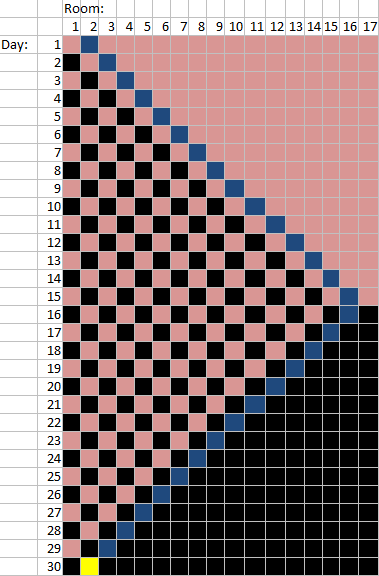
\includegraphics[width=0.5\linewidth]{images/princess-problem.png}
\end{figure}
\end{solution}

% https://cemc.uwaterloo.ca/events/mathcircles/2013-14/Fall/Junior78_Nov19.pdf
% https://www.math.cmu.edu/~mlavrov/arml/12-13/games-02-24-13.pdf
% https://math.mit.edu/research/highschool/primes/materials/2015/Ji-Park-Song.pdf
% https://mathcircle.berkeley.edu/sites/default/files/archivedocs/2015/lecture/BMC_Int2-Sep1-2015-combinatorialgames.pdf